\documentclass[12pt, a4paper]{article}

\usepackage[brazilian]{babel}
\usepackage[utf8]{inputenc}
\usepackage[T1]{fontenc}
\usepackage{url}
\usepackage[backend=biber,style=abnt]{biblatex}
\usepackage[autostyle]{csquotes}
\usepackage{authblk}
\usepackage[a4paper, left=3cm, right=2cm, top=3cm, bottom=2cm]{geometry}
\usepackage{setspace}
\usepackage{multirow}
\usepackage{listings}
\usepackage{graphicx}
\usepackage{subcaption}

\onehalfspacing

\addbibresource{artigo.bib}

\author{Gabriel Almeida Bueno}
\affil{FATEC Zona Sul}
\title{Tecnologia e Artes, um estudo sobre a tecnologia da informação como meio para compreensão e realização artística}

\begin{document}

\maketitle

\section{Introdução}
% O que é arte? Qual é a sua importância?
A arte é parte indissociável da vivência humana, e a tecnologia é parte indissociável da arte. 
Sendo uma das atividades mais antigas exercidas pelo ser-humano, podemos enxergar características estéticas e manifestações artísticas realizadas pelos vários povos e culturas antigas até a contemporaneidade, seja por meio do artesanato, arquitetura, pintura ou poesia.
O belo sempre é benquisto por qualquer indivíduo que seja, independente do seu meio social ou seus gostos pessoais.
Na Poética, ao definir a arte da poesia, Aristóteles \cite[p.42]{aristotle_poetics} afirma que 

\begin{displayquote}
as coisas que observamos ao natural e nos fazem pena agradam-nos quando as vemos representadas em imagens muito perfeitas.
\end{displayquote}

Cada registro artístico, porém, representa não só algo que é sensivelmente belo, mas constitui uma expressão do indivíduo que a fez, carregando em si
também o espírito da época em que foi realizado, do meio em que o artista estava inserido. 
A arte mostra-se, portanto, de valor inestimável como registro da expressão humana, Da Vinci \cite{davinci_thoughtsonart} diria que:

\begin{displayquote}
Os frutos da pintura podem ser compreendidos por todas as populações do universo pois seus resultados
são sujeitos ao poder da visão [...] não necessitando de intérpretes para as várias línguas.
\end{displayquote}

Identidades religiosas e nacionais também fazem uso da estética, já que historicamente podemos observar que, nas palavras de Hegel \cite{hegel}:

\begin{displayquote}
é nos trabalhos de arte que nações tem depositado as mais ricas intuições e ideias que possuem; e não 
infrequentemente as belas artes fornecem uma chave para a interpretação da sabedoria e religião dos povos.
\end{displayquote}

Já o ato de realizar arte, por outro lado, é estritamente ligado à tecnologia.
As ferramentas criadas pelo homem a fim de subjugar os obstáculos impostos
pelo meio ambiente à sua sobrevivência, foram e sempre serão usadas pelo artista como meio de expressão e para o fazer artístico \cite{gouzouasis}.
A evolução da tecnologia interfere diretamente nas manifestações artísticas, o que podemos notar pela simples observação da arte ao longo da história: das pinturas que passaram das paredes das cavernas para o óleo em tela, até
a fotografia; da música tocada em alaúdes com tripas torcidas que passou para os violões com cordas de nylon, até as guitarras elétricas; 
da gravação e reprodução sonora que partiu do fonógrafo até os computadores e CDs, até o mais recente \emph{streaming}. 
É notório como a tecnologia de uma época pode influenciar nas manifestações artísticas do período. 

Um dos sentidos que o famoso aforismo de McLuhan, "o meio é a mensagem", carrega em si é o de que o 
\emph{meio transforma o seu conteúdo} \cite[p.50]{braga_mcluhan}. 
Um novo meio, fruto de uma inovação tecnológica, impacta na própria mensagem passada na obra artística.
Estamos na era da informação, com capacidade computacional de sobra e uma digitalização crescente do mundo tangível. 
Como a tecnologia contemporânea pode influenciar no estado atual da realização e compreensão artística?

\begin{figure}[ht!]
	\centering
	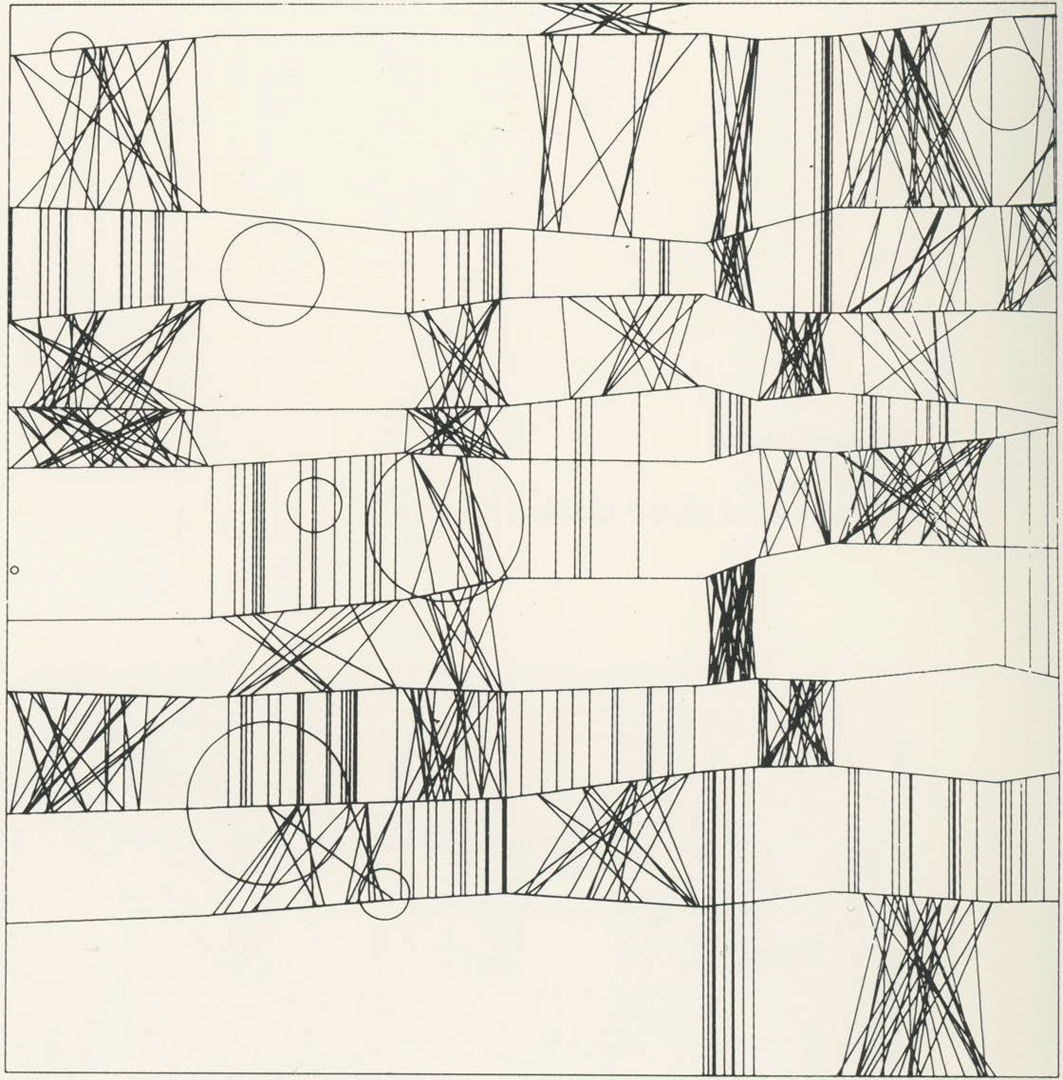
\includegraphics[width=\textwidth, height=7cm, keepaspectratio=true]{fig/hommage_to_paul_klee}
	\caption{
		Obra \emph{Hommage à Paul Klee}, de Frieder Nake, realizada em 1965 \cite{homage_to_paul_klee}.
	}
\end{figure}

\begin{figure}[ht!]
	\centering
	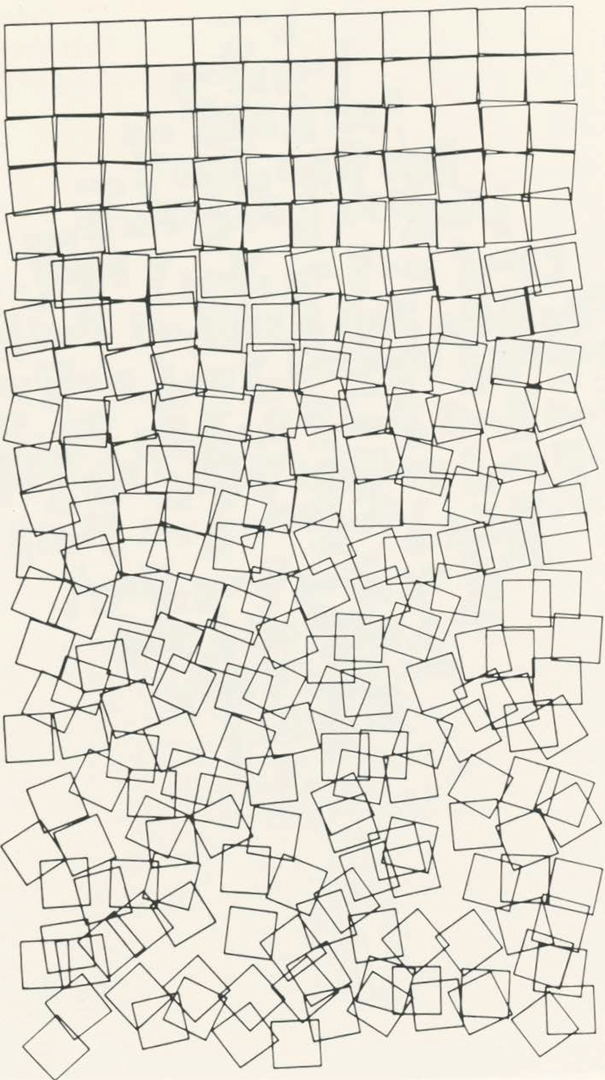
\includegraphics[width=\textwidth, height=7cm, keepaspectratio=true]{fig/gravel_stones}
	\caption{
		\emph{Gravel Stones}, de Georg Nees
		\cite{gravel_stones}.
	}
\end{figure}

Como exemplos do fazer artístico utilizando como meio a tecnologia contemporânea, podemos ressaltar o trabalho
de artistas como Frieder Nake, Georg Nees e Vera Molnar que, em meados dos anos 60, influenciados pela filosofia de Max Bense, vanguardearam 
o movimento da arte algorítmica, conhecido também pelas alcunhas de arte generativa, arte computacional, gráficos generativos, entre outros.
O algoritmo é a principal ferramenta do artista computacional, através do qual a ideia da obra artística é modelada em um programa de computador -- utilizando-se de símbolos, eventos e estados -- que ao ser executado produzirá a obra em si. Neste movimento, o modo convencional do fazer artístico, já conhecido a muito, dá lugar para a ciência e a matemática. 

Vemos que a tecnologia contemporânea já é tão significativa que nos deu novos meios para o fazer artístico, trazendo consigo, além disso, reflexões acerca do próprio ato de fazer arte, já que a ideia de arte feita "pelo computador" não é aceita de bom grado pelo crítico
mais conservador.
Ora, não há de se negar que o matemático, cientista ou engenheiro mais romântico, apesar de não necessariamente chamar de arte, indubitavelmente enxerga alguma forma de beleza na atividade que exerce e nos frutos de seu trabalho. 
Na sua apologia, Hardy \cite{hardy_apology} escreve:

\begin{displayquote}
Um matemático, como um pintor ou poeta, é um criador de padrões. Se os padrões daquele são mais permanentes do que os destes, é porque eles são feitos com ideias.
\end{displayquote}

Ao lamentar a forma como a matemática é ensinada para as crianças em nível escolar (sua lamentação poderia muito bem ser transposta para o próprio ensino de arte), Lockhart \cite{lockhart_lament} expressa que:

\begin{displayquote}
Nenhuma sociedade jamais reduziria uma forma tão bela e significativa de arte para algo tão insignificante e trivial. Nenhuma cultura poderia ser tão cruel com suas crianças a ponto de privá-las de um meio tão satisfatório e natural de expressão humana.
\end{displayquote}

A sociedade cada vez mais vê-se de todo tomada pela digitalização. Se o homem se torna digital, sua expressão em forma de 
manifestação artística se tornará, também, digital. Como isso impactará no ensino vigente da arte?
Há a necessidade de se apresentar ao aluno a tecnologia contemporânea como forma de realização e estudo da arte.
Os três pilares da abordagem triangular de Ana Mae Barbosa -- o conhecimento da história, a apreciação da arte, e o próprio fazer artístico --
deveriam ser extendidos para abranger também a arte produzida pelos meios contemporâneos ao aluno.
É evidente que a tecnologia não é uma panaceia para resolver todos os problemas da educação artística, porém, a tecnologia atual, já que é parte
inseparável do indivíduo, deve, de alguma forma e em algum momento, nem que breve, ser abordada a fim de contextualizá-lo na sociedade em que vive.

Tendo em vista esta natureza inerentemente tecnológica da arte, em contraponto com a aparente falta de diálogo entre o meio artístico e o campo
mais recente do desenvolvimento tecnológico -- algo que pode ser observado empiricamente em certos meios -- este trabalho apresenta-se com o objetivo
de relacionar uma das tecnologias que mais vem recebendo atenção dos pesquisadores e engenheiros -- a das inteligências artificiais, mais especificamente,
o das \emph{redes neurais} -- com o meio da arte. 
Uma breve revisão das inteligências artificiais e das redes neurais será feita a fim de, para contextualizar o assunto, criar uma base 
histórica e teórica do assunto, além de citar outros trabalhos realizados na área que possuem alguma relação com a arte.
Como estudo de caso e exemplo de aplicação prática, um sistema de rede neural capaz de tentar categorizar o estilo artístico
de uma pintura foi criado. Este sistema mostra uma possível forma de integração de uma rede neural com o meio artístico, 
abrindo ainda mais possibilidades para a criação e evolução de sistemas de informação na arte, seja como ferramenta para auxílio a educação ou para a própria realização artística. 
Para tentar detectar o interesse popular da abordagem de tecnologia no ensino artístico, como uma forma de testar a hipótese de
que é necessário pelo menos uma abordagem eventual da tecnologia recente na arte, uma pesquisa foi conduzida com aproximadamente 70 pessoas. Seus resultados
também serão exibidos neste trabalho.

\section{Referencial teórico}
\subsection{Uma breve história da IA e das Redes Neurais}
\subsection{Redes Perceptron}
\subsection{Redes Neurais Convolucionais (CNNs)}
\subsection{Redes Neurais Adversariais (GANs)}
\subsection{Transferência de Aprendizado}
\subsection{Frameworks atuais para o treinamento de Redes Neurais}

% \nocite{*}
\printbibliography

\end{document}